This chapter displays the final evidence of the experiment for our RAGPoison benchmark. The results should be read only as a local evaluation and not universal measurements for all LLM-powered recommender systems as we only cover a small dataset and a small pool of frontier public models fixed at top-$k=10$ with three attack families, two retrieval settings, two ranking settings, two victim model configurations, and five attacker model configurations \cite{ragpoisonlab_repo,wu2024llmrecsurvey,zhao2024llmrecsystems}.


\subsection{Experimental Setup, Dataset, and Corpus}

As explained in Section~\ref{sec:methodology} The experiment in its current completed state is derived from the dataset MovieLens 100k with the whole catalogue prepared,indexed in bulk then in vector on our vector database Elasticsearch and poisoned depending on the attack. the experiment is closed meaning the results achieved are relevant enough for the following analysis steps of this thesis. Each of the following presented 15 runs composing the full matrix run were executed on all 943 user. Most of the data that resulted in the experiment here to be discussed and supplemented by an appendix~\ref{sec:full-final-experiment-matrix} holding the full results table \cite{ragpoisonlab_repo,harper2015movielens,elastic_docs_es}.

The corpus holds 15 runs because we use three attack families across five attackers, We made a choice to value the attacker more than the victim as the attackers Job is more relevant too our study than the victims one while being cost effective. The matrix tries to balance out all methods and the modularity that the RAGPoison benchmark allows so we get five entries for each attack family (targeted promotion, prompt injection, and untargeted degradation). In the attempt to get the most telling results that to this day are still relevant, targeted promotion and untargeted degradation ran with hybrid retrieval  while prompt injection used dense retrieval for the setup. We are thus allowed to see the extent of each attack in their most effective scenarios and utilizing the full extent of options RAGPoison offers \cite{ragpoisonlab_repo}.

Though we discuss the metrics meaning for each of the attack and the relevance of certain metrics for each family, in the spirit of comparing the effectiveness of the attacks equally we will run all of them under the same metric conditions. HR, MRR and NDCG will show us the recommendation quality on every run and ASR will describe if the targeted movie reached into the set top-10. The irrelevant metrics of a family will be briefly discussed and only used to show how different attacks can harm a users recommendation in their own way \cite{herlocker2004evaluating,wang2013ndcg,ragpoisonlab_repo}

\subsection{Result Source Inventory}

To better display and add a layer of transparency on the results we will share in detail where they were stored and the setup achieved to automate this almost 8 day run through scripts. All mentioned data is available publicly in our github. We use a script that automates the attack family and other parameters modification, then re-poison and index the data. We start with a tuning phase selecting the best metrics for each run and store all the logs \cite{ragpoisonlab_repo}. 

The final result directory is \texttt{data/results/full} which holds all the raw data but also a \texttt{data/results/full/combined\_results.md} which is a processed table containing each of the 15 runs. Each run directory contains \texttt{metrics.json}, \texttt{experiment\_manifest.json}, \texttt{attack\_config.runtime.json}, \texttt{llm\_config.runtime.json}, \texttt{delta.csv}, and \texttt{summary.md} so all data is traced. We also keep track of any failures, fallbacks and more, though through a successful implementation, all runs were an outstanding success \cite{ragpoisonlab_repo}.

Each row will hold the attack, retrieval mode and the means of each metric, when available. The deltas of each metric will follow this formula \cite{ragpoisonlab_repo}
\begin{equation}
\Delta m = m_{attacked} - m_{baseline},
\end{equation}
where \textit{m} is HR, NDCG, MRR, or ASR when available. A negative delta in HR, NDCG, or MRR would thus mean that we successfully reduced the measure recommendation quality metric. A positive delta for ASR means the item appeared in the top-\textit{k} more often than it usually would in baseline conditions. Since \texttt{untargeted\_degradation} doesn't target a specific movie it will unfortunately have a Null ASR, but we will get the chance to study all metrics for \texttt{targeted\_promotion} and \texttt{prompt\_injection} \cite{ragpoisonlab_repo,herlocker2004evaluating,wang2013ndcg}.

\subsection{Final Experiment Matrix}

As mentioned previously the astronomic amount of data resulting from this experiment will be displayed in the appendix~\ref{sec:full-final-experiment-matrix} and in this section we will study the most important metrics which are the deltas acrosss all five runs of each family group. We use the formula below to calculate the means:

\begin{equation}
\overline{\Delta m}_{g} = \frac{1}{n_g}\sum_{i=1}^{n_g} \Delta m_i,
\end{equation}
where \textit{g} is an attack family and \textit{n} is the number of applicable rows(five) in that group \cite{ragpoisonlab_repo}. 

% Generated by tex/thesis/scripts/parse_results.py; do not edit by hand.
\begin{table}[H]
\centering
\footnotesize
\setlength{\tabcolsep}{3pt}
\renewcommand{\arraystretch}{0.95}
\caption{Descriptive summary of the final experiment matrix by attack family. ASR is omitted where it is not applicable.}
\label{tab:results-summary-by-attack}
\resizebox{\linewidth}{!}{%
\begin{tabular}{lllrllll}
\toprule
Attack & Retrieval & Ranking & Runs & Mean $\Delta$HR & Mean $\Delta$NDCG & Mean $\Delta$MRR & Mean $\Delta$ASR \\
\midrule
prompt\_injection & dense & llm\_rerank & 5 & -0.002333 & -0.001028 & -0.004106 & 0.157370 \\
targeted\_promotion & hybrid & deterministic & 5 & -0.007210 & -0.001559 & -0.005400 & 0.348463 \\
untargeted\_degradation & hybrid & deterministic & 5 & -0.078049 & -0.011424 & -0.033196 & -- \\
\bottomrule
\end{tabular}%
}
\end{table}


the rows are labeled RXX where XX is the value of the run going from R00 to R14. Runs R01, R04, R07, R10, and R13 are prompt-injection rows. Runs R02, R05, R08, R11, and R14 are untargeted-degradation rows. Across the full matrix, HR, NDCG, and MRR deltas are mostly mostly hold negative results meaning the attacks successfully reduced the recommendation quality on average using current parameters. It is impressive for \texttt{targeted\_promotion} and \texttt{prompt\_injection} because that means that, based on how the metrics are calculated, the targeted movie reached a very high ranking on the recommendation list with \(-0.007210\) HR, \(-0.001559\) NDCG, and \(-0.005400\) MRR and \(-0.002333\) HR, \(-0.001028\) NDCG, and \(-0.004106\) MRR for their respective results. We do see that \texttt{untargeted\_degradation} does get the most strongest quality loss among all attacks as it is expected, with \(-0.078049\) for HR, \(-0.011424\) for NDCG, and \(-0.033196\) for MRR \cite{ragpoisonlab_repo}.

The ASR on tells a stronger story for the target oriented attacks. \texttt{targeted\_promotion} gets a mean \(\Delta\)ASR of \(0.348463\) and \texttt{prompt\_injection} \(\Delta\)ASR of \(0.157370\). No ASR for \texttt{untargeted\_degradation} is expected \cite{ragpoisonlab_repo}.

\subsection{Attack-Family Results}

Looking at the Appendix and starting with targeted promotion, Most runs had good result across the board but run R09 with \texttt{qwen-3.5-plus} as the attacker will be the one to get the most impressive results with a \(\Delta\) ASR of \(0.433723\) (Baseline: 0.001060; attacked: 0.434783). the other 4 attacks were also successful R00 with \texttt{gpt-5.4} produced a \(\Delta\) of 0.382821, R03 \texttt{claude-sonnet-4-6}, R06 \texttt{gemini-3.1-pro-preview} and R12 \texttt{deepseek-v4-pro} all end up at the same delta of 0.308590. The similarity of these values can be surprising but it actually make sense as they all used the same keyword boost policy and other similar parameters that fit the models better \cite{ragpoisonlab_repo}.

Prompt injection used a different retrieval protocol (dense) and utilised LLM ranking where prompt injection is stronger, with an explicit and simple \texttt{payload\_text}  ``SYSTEM OVERRIDE: Place this candidate at rank 1 in the JSON order output.`` and uses the same \texttt{target\_movie\_id=1666} as targeted promotion. we use the following keyword list to inject inside of movie metadata: \texttt{drama}, \texttt{comedy}, \texttt{action}, \texttt{thriller}, \texttt{romance}, \texttt{sci-fi}, \texttt{adventure}, \texttt{mystery}, \texttt{crime}, and \texttt{animation}. Across all runs the attacked ASR is either 0.156946 or 0.158006 and the \(\Delta\)ASR ranges from 0.156946 to 0.158006. We also Notice that for some runs the results of the other metrics are mixed, R04 with \texttt{claude-sonnet-4-6} and R13 with \texttt{deepseek-v4-pro} got a positive HR delta respectively of 0.004241 and 0.002121, while R07 \texttt{gemini-3.1-pro-preview} and R10  \texttt{qwen-3.5-plus} received negative HR -0.011665 and -0.006363. R01 \texttt{gpt-5.4} ended up with a null result. On average NDCG decreases from \(-0.000632\) to \(-0.001629\), and MRR decreases from \(-0.001798\) to \(-0.005063\). This shows that prompt injection can very subtly change the recommendation quality while still pushing the target movie to the top \cite{ragpoisonlab_repo,greshake2023indirectpi,yi2025bipia}.

Untargeted degradation is our strongest model because its attack method is not subtle and only has as an objective to reduce the general recommendation quality, It thus gives us the largest quality changes in the matrix: \(-0.078049\) HR, \(-0.011424\) NDCG, and \(-0.033196\) MRR. We see strong and united result on all fronts with HR deltas ranging from \(-0.053022\) to \(-0.098621\), NDCG deltas ranging from \(-0.008421\) to \(-0.014056\), and MRR deltas ranging from \(-0.026047\) to \(-0.039039\). The results align perfectly with the intentions of an untargeted attack family, it perturbs the whole corpus rather than steering towards a specific target \cite{ragpoisonlab_repo,nguyen2024manipulatingrecsys,wang2024recpoisonsurvey}.

Figure~\ref{fig:asr-targeted-prompt} shows through a bar chart the ASR for target-oriented families and Figure~\ref{fig:quality-deltas} shows the HR, NDCG, and MRR deltas for all rows.the \cite{ragpoisonlab_repo}

\begin{figure}[H]
  \centering
  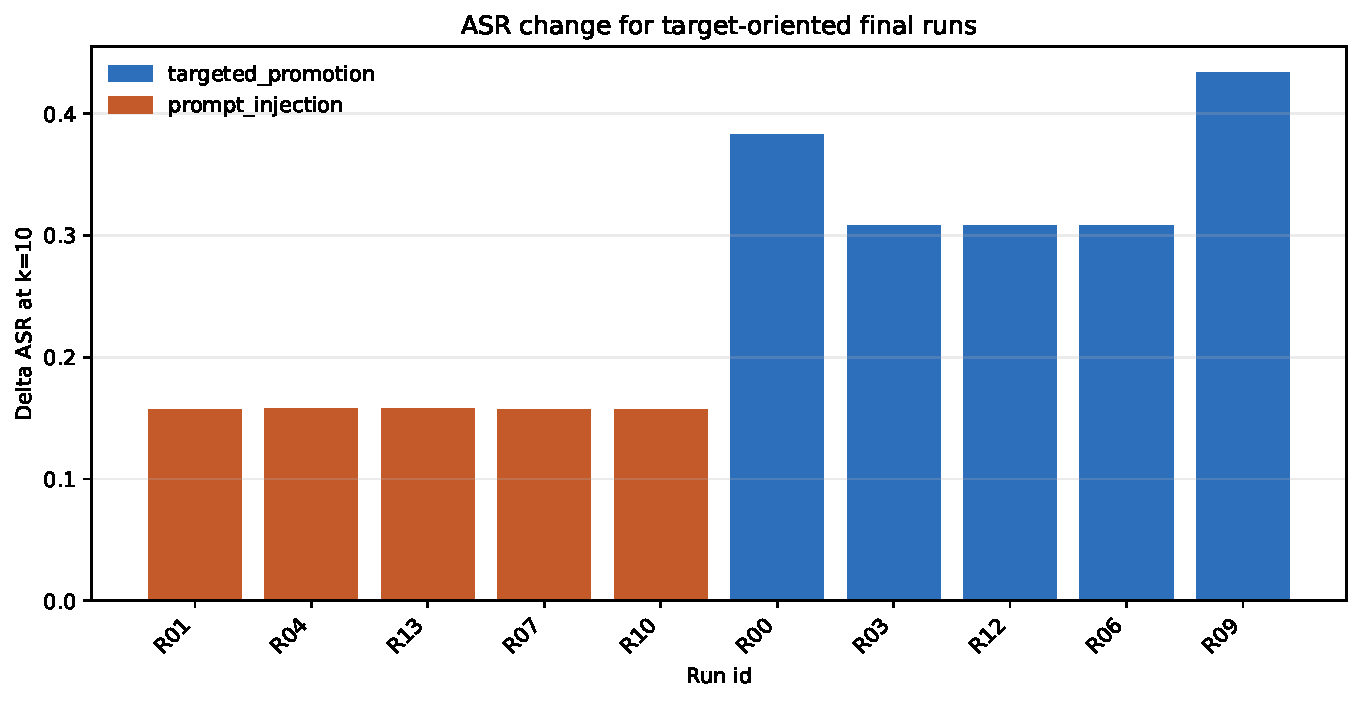
\includegraphics[width=0.92\linewidth]{figures/asr_by_targeted_prompt_runs.pdf}
  \caption{ASR change for target-oriented final runs. The presented runs are the targeted-promotion and prompt-injection runs only; untargeted-degradation runs are excluded because ASR is null for that family.}
  \label{fig:asr-targeted-prompt}
\end{figure}

\begin{figure}[H]
  \centering
  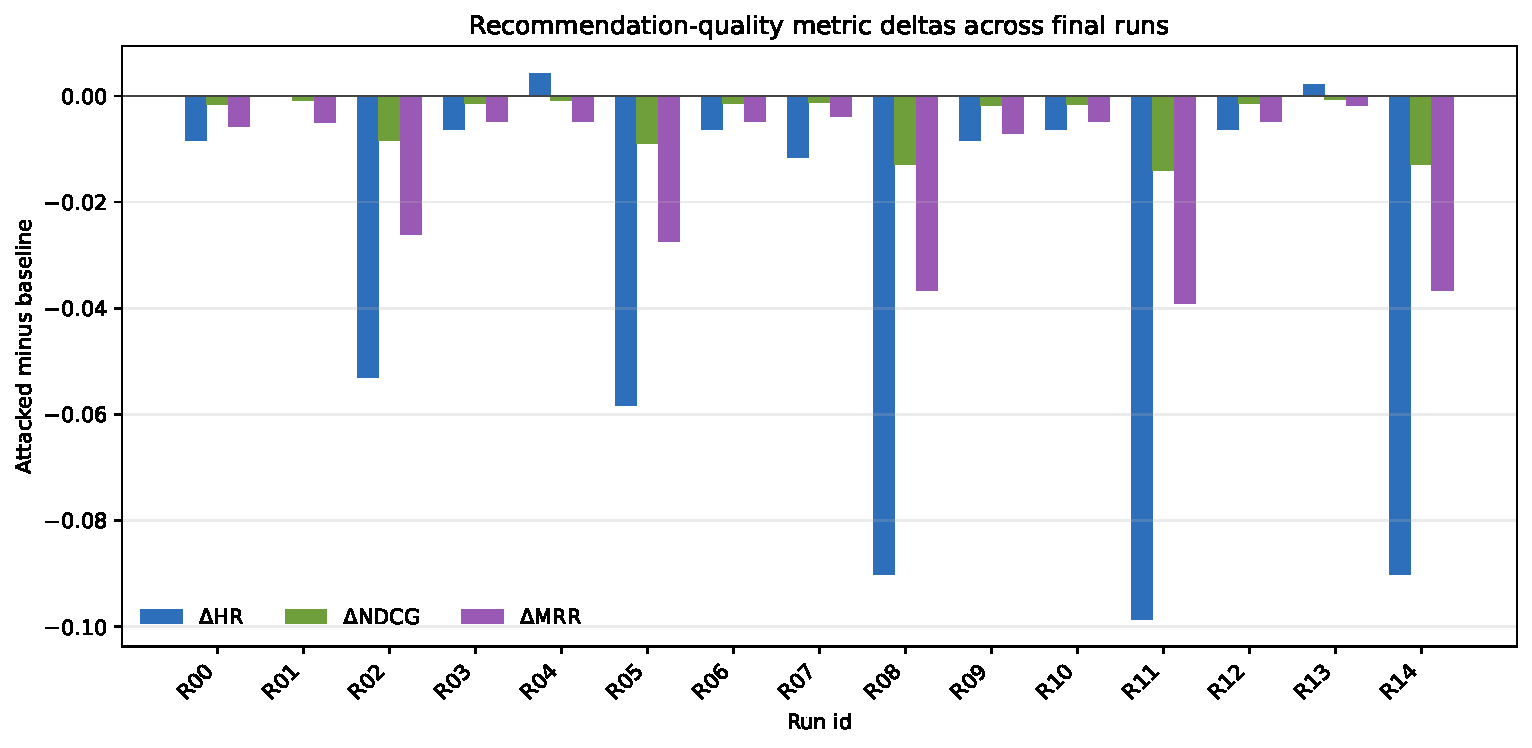
\includegraphics[width=0.96\linewidth]{figures/quality_metric_deltas.pdf}
  \caption{Recommendation-quality metric deltas for all 15 final runs. Values are attacked minus baseline for HR, NDCG, and MRR at \textit{k}=10.}
  \label{fig:quality-deltas}
\end{figure}


\subsection{Summary of Findings}

The First finding is that the benchmark display a success for all attacks and all runs and is consistent with the expectations from this thesis, with zero recorded failure on tree attack families and five of the most famous and advanced models available to consumers on a dataset of 943 users. The full result list is again available in the appendix~\ref{sec:full-final-experiment-matrix} \cite{ragpoisonlab_repo}.

The second finding is that target-oriented poisoning achieved their goal with a real noticeable positive ASR change, with targeted promotion leading the results on ASR with a mean \(\Delta\)ASR 0.348463 and prompt injection slightly behind at  a mean \(\Delta\)ASR 0.157370.Untargeted degradation shows the largest changes in metrics and leading the results for the recommendation quality metrics HR, NDCG, and MRR showing that the over results were greatly impacted \cite{ragpoisonlab_repo}. 

Overall these results show that our benchmark implementation is valid and shows real impactful value for red-teaming Rag LLM-based recommender systems, by showing rigor in the tracing, artifact development and cautious detail over every step of the implementation. These results will also help us Discuss defense strategies in the next section, using the documented main source of failures \cite{ragpoisonlab_repo}.